Ziel des Versuches ist es, den Brechungsindex und die Dispersionskurve eines Gases zu bestimmen.
Dies geschieht mit Hilfe eines Prismas, einer Cadmium-Quecksilber-Lampe, eines Fernsrohs und eines Winkelmessers, die wie in Abbildung~\ref{fig:aufbau} gezeigt angeordnet sind. Die Lampe ist fest. Vor ihr ist auf einer drehbaren Platte mit Winkelanzeige das Prisma angebracht. Ein Fernrohr ist darum herum schwenkbar. \\

\begin{figure}[h!]
	\centering
	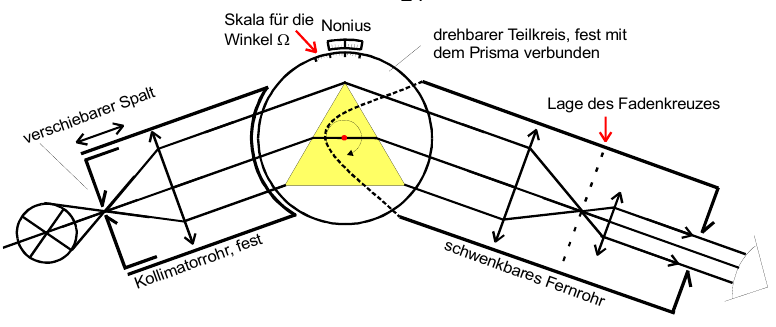
\includegraphics[width=0.8\textwidth]{Aufbau.png}
	\caption{Versuchsaufbau}
	\label{fig:aufbau}
\end{figure}

An dem Prisma wird der Lichtstrahl doppelt gebrochen. Zur Berechnung des Brechungsindex ist zum einen der Winkel  $\eta$ zwischen eingehendem und ausgehendem Stahl relevant zum anderen der Innenwinkel $\varphi$ des Prismas. Wobei hier ein gleichseitiges Prisma vorliegt. Mit Hilfe des Snelliusschen Gesetz \eqref{eq:snellius}, das auf eine Doppelbrechung, wie in Abbildung~\ref{fig:prisma1} dargestellt, angewendet wird, folgt der Brechungsindex
\begin{align}\label{BrechIndex}
	n=\frac{\sin\frac{\eta + \varphi}{2}}{\sin\frac{\varphi}{2}} \quad .
\end{align}

\begin{figure}[h!]
	\centering
	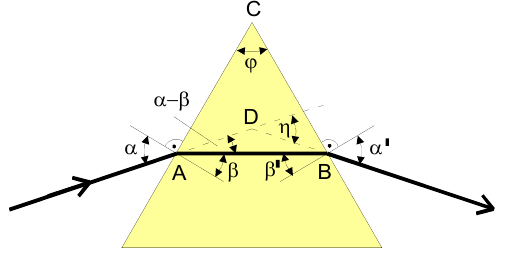
\includegraphics[width=0.7\textwidth]{Prisma1.png}
	\caption{Doppelbrechung am Prisma}
	\label{fig:prisma1}
\end{figure}

\clearpage

\subsection{Messung des Innenwinkels $\varphi$}
Zur Messung des Innenwinkels $\varphi$ wird das Prisma so ausgerichtet, dass eine Spitze auf die Lampe zeigt und dann unverändert in dieser Position gelassen. Durch das Fernglas wird eine Spektrallinie der Lampe, die auf der Prismenoberfläche zu sehen ist erst auf der einen Seite des Prismas, dann auf der anderen Seite anvisiert. Jeweils wird der Winkel $\varphi_r$ bzw. $\varphi_l$ notiert. Aus Abbildung \ref{fig:prisma2} folgt mit einfacher Trigonometrie
\begin{align}\label{Phi}
	\varphi = \frac{1}{2} (\varphi_r - \varphi_l) \quad.
\end{align}

\begin{figure}[h!]
	\centering
	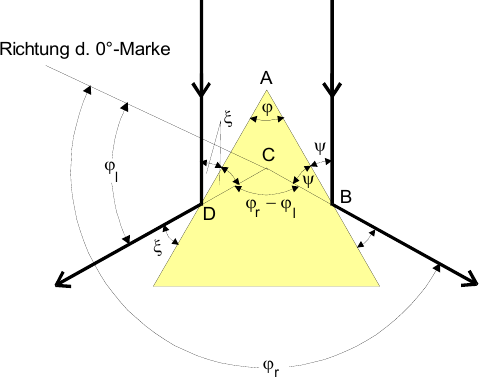
\includegraphics[width=0.42\textwidth]{Prisma2.png}
	\caption{Innenwinkelmessung}
	\label{fig:prisma2}
\end{figure}

\subsection{Messung des Brechungswinkels $\eta$}
Im Gegensatz zur Messung des Innenwinkels wird bei der Bestimmung des Brechungswinkels das Prisma rotiert und das Fernrohr an einem festen Ort gelassen. \\
Fernrohr und Prisma werden einmalig so ausgerichtet, das die Spektrallinien zu sehen sind. Eine Linie wird ausgewählt und beobachtet. Dann wird das Prisma so lange gedreht, bis dieselbe Spektrallinie wieder im Fadenkreuz des Fernrohres liegt. Die Winkel beider Einstellungen $\Omega_r$ und $\Omega_l$ dienen zur Berechnung der Brechungswinkels $\eta$
\begin{align}\label{Eta}
	\eta = 180 - (\Omega_l - \Omega_r) \quad .
\end{align}
Der Vorgang ist in Abbildung \ref{fig:prisma3} dargestellt.

\begin{figure}[h!]
	\centering
	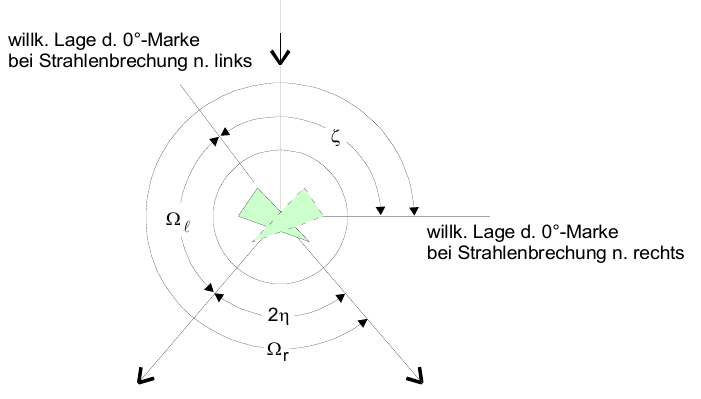
\includegraphics[width=0.57\textwidth]{Prisma3.png}
	\caption{Brechungswinkelmessung}
	\label{fig:prisma3}
\end{figure}

